
The requirement for a $\epsilon$-orthogonal group (semi-orthogonal user selection group, or SUS group) is broken into two parts. Firstly the users in the group are required to have a channel norm similar to other users in the group. This upper and lower bound on SNR ensures that users in an SUS group with high channel gain do not excessively interfere with low-SNR users in the group. The lower SNR bound ensures a minimum quality of service for users in the group. The second part of the requirement addresses interference in terms of channel orthogonality. The expression for a SUS group requirements is given by as

\begin{equation}\label{eq:S_e}
    \begin{aligned}
        \mathcal{S}_\epsilon = \lbrace \mathcal{S}_a \big|\ | \textbf{h}_i\textbf{h}_j^H |\ <\ \epsilon \ \text{;} \ \rho^-<\Vert \textbf{h}_i \Vert^2 < \rho^+\ \forall \ i \neq j \in \mathcal{S}_a \rbrace
    \end{aligned}
\end{equation}

Swannack develops a lower bound on the probability of existence of an SUS group, more precisely: $Pr[\mathcal{S}_\epsilon \neq \lbrace \emptyset \rbrace]$. Existence probability depends on the orthogonality requirements given in \ref{eq:S_e}, the group size $l = \mathcal{S}_a$, and the number of users that have be considdered for addition to the SUS group $n$. Swannack considers an example to illustrate results. The example is shown in Fig. \ref{fig:swannack_fig5a}, this example was replicated with results of replication shown in Fig. \ref{fig:reproduce_fig5a}. The purpose of this example is to deterimine the number of users that must be evaluated for addition to an SUS group of size 2, 3, and 4 to achieve a probability of existence of 90\%. In this example 4 transmit antennas are assumed.

\begin{figure}
    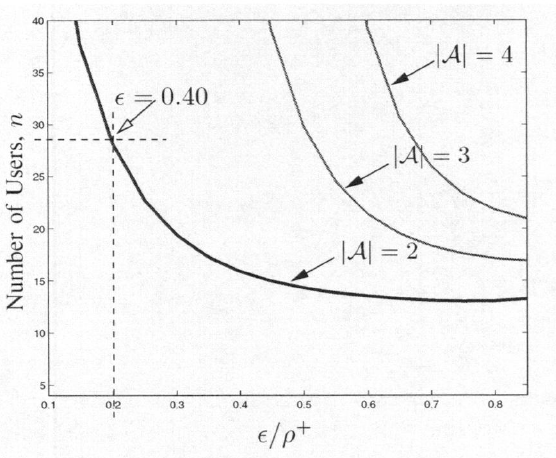
\includegraphics[width=12cm]{figs/swannack_fig5a.png}\\
    \caption{Plot of minimum number of users to achieve minimum probability of SUS group existence of 0.9. 4 transmit antennas are assumed for all curves.}
    \label{fig:swannack_fig5a}
\end{figure}

\begin{figure}
    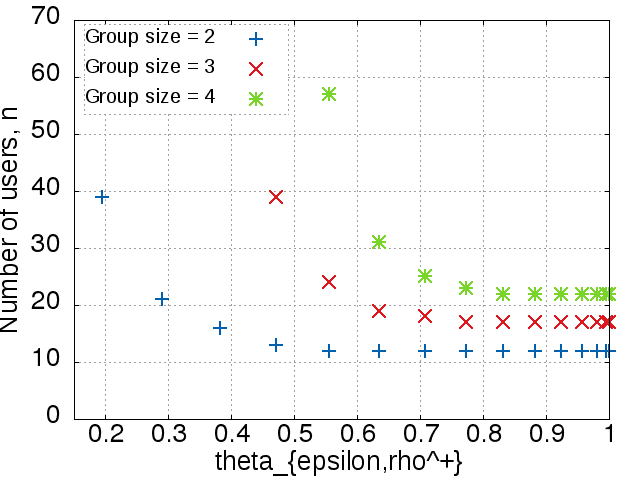
\includegraphics[width=12cm]{figs/existence.png}\\
    \caption{Plot of minimum number of users to achieve minimum probability of SUS group existence of 0.9. 4 transmit antennas are assumed for all curves. Horizontal axis scale is $\cos{(\theta_\epsilon,\rho^+)} = \frac{\epsilon}{\rho^+}$}
    \label{fig:reproduce_fig5a}
\end{figure}

\subsection{Extending results to relaxed, widely linear orthogonality constraint}

We now consider relaxing the orthogonality constraint to consider only the real part of the channel inner product:
\begin{equation}\label{eq:wl_S_e}
    \begin{aligned}
        \mathcal{S}_\epsilon = \lbrace \mathcal{S}_a \big|\ \mathfrak{Re} \lbrace \textbf{h}_i\textbf{h}_j^H \rbrace\ <\ \epsilon \ \text{;} \ \rho^-<\Vert \textbf{h}_i \Vert^2 < \rho^+\ \forall \ i \neq j \in \mathcal{S}_a \rbrace
    \end{aligned}
\end{equation}

Changing orthogonality requirement to consider only the real part of the inner product between channels is expected to impact the probability of existence both in terms of SNR and SIR. Swannack offers a geometric interpretation of the channels existing in complex $m$-space, where $m$ is the number of transmit antennas.

The geometric analog of user $i$'s channel, $\textbf{h}_i$, satisfying the SNR requirement is that $\Vert\textbf{h}_i\Vert^2$ lies in the spherical 2$m$ shell between $\rho^-$ and $\rho^+$. The geometric analog of the orthogonality requirement is that the angle formed between any two channels in the SUS group are greater than $\arccos{(\frac{\epsilon}{\rho^+})}$.

In the complex-channel case presented by Swannack, the probability that the channel satisfies SNR requirements is given by:
\begin{equation}\label{eq:p_s}
    \begin{aligned}
        p_s = \Gamma(2m,m\rho^-) - \Gamma(2m,m\rho^+)
    \end{aligned}
\end{equation}

TODO: Consider derivation of $p_s$, and make changes to real case. Shouldn't be too bad: assumption in the above is that $\textbf{h}_i$ is circular-symmetric complex Gaussian.

\begin{equation}\label{eq:p_perp}
    \begin{aligned}
        p_\perp \geq (1-(1-l)\delta_c(\theta_{\epsilon,\rho},2m))^{l-1}
    \end{aligned}
\end{equation}

\begin{equation}\label{eq:delta_c_sphere}
    \begin{aligned}
        \delta_c(\theta,2m) = 2\frac{\Omega_{2m}(\theta)}{\Omega_{2m}(\pi)}
    \end{aligned}
\end{equation}

\begin{figure}
    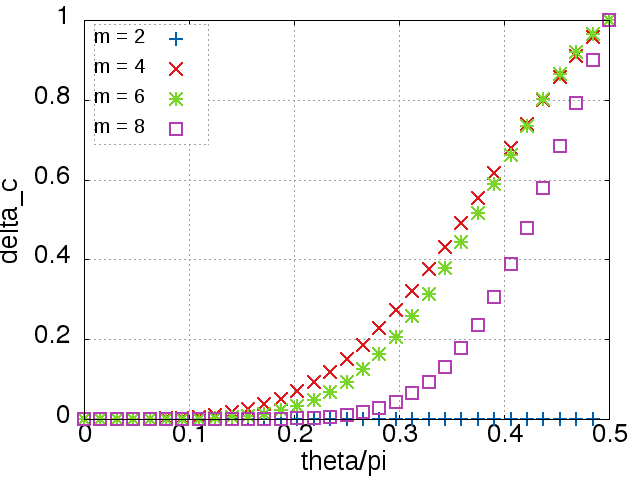
\includegraphics[width=12cm]{figs/delta.png}\\
    \caption{Plot of $\delta_c$ as a function of $\theta_{\epsilon,\rho}$ over various dimensions (ie. number of transmit antennas)}
    \label{fig:delta}
\end{figure}

\begin{figure}
    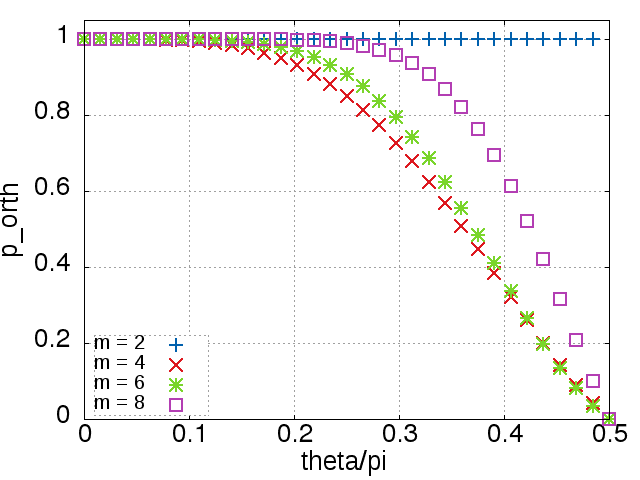
\includegraphics[width=12cm]{figs/p_orth_gs_2.png}\\
    \caption{Plot of $p_{\perp}$ as a function of $\theta_{\epsilon,\rho}$ over various dimensions (ie. number of transmit antennas), SUS group size of 2}
    \label{fig:p_orth_gs_2}
\end{figure}

\begin{figure}
    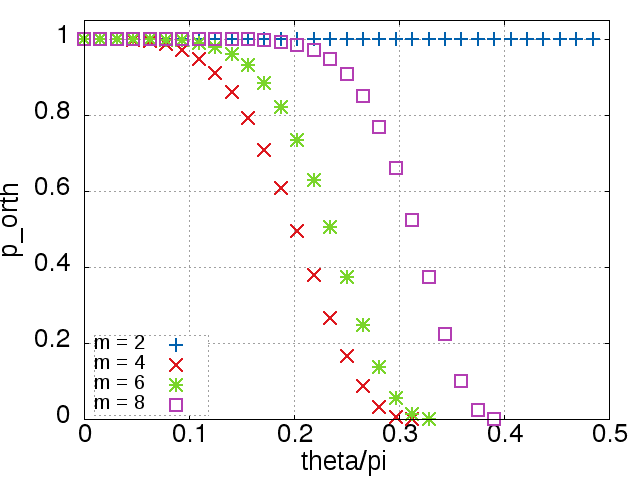
\includegraphics[width=12cm]{figs/p_orth_gs_4.png}\\
    \caption{Plot of $p{\perp}$ as a function of $\theta_{\epsilon,\rho}$ over various dimensions (ie. number of transmit antennas), SUS group size of 4}
    \label{fig:p_orth_gs_4}
\end{figure}

\begin{figure}
    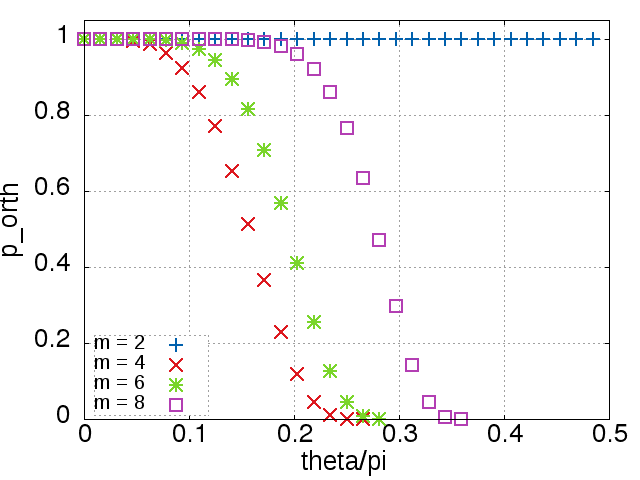
\includegraphics[width=12cm]{figs/p_orth_gs_6.png}\\
    \caption{Plot of $p{\perp}$ as a function of $\theta_{\epsilon,\rho}$ over various dimensions (ie. number of transmit antennas), SUS group size of 6}
    \label{fig:p_orth_gs_6}
\end{figure}

\begin{figure}
    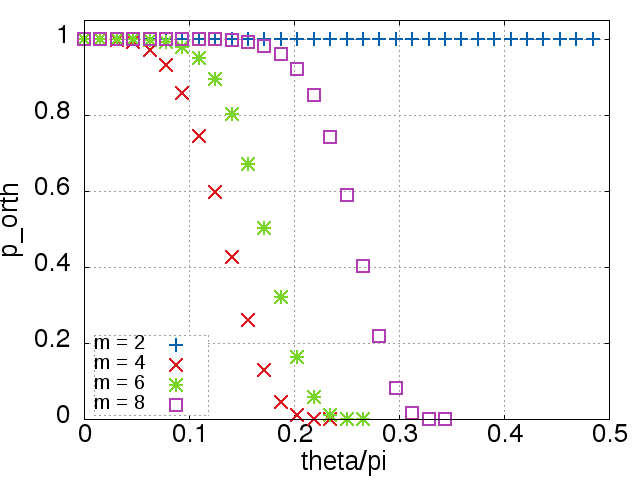
\includegraphics[width=12cm]{figs/p_orth_gs_8.png}\\
    \caption{Plot of $p{\perp}$ as a function of $\theta_{\epsilon,\rho}$ over various dimensions (ie. number of transmit antennas), SUS group size of 8}
    \label{fig:p_orth_gs_8}
\end{figure}